%%%%%%%%%%%%%%%%%%%%%%%%%%%%%%%%%%%%%%%%%%%%%%%%
%% Intro to LaTeX and Template for Homework Assignments
%% Quantitative Methods in Political Science
%% University of Mannheim
%% Fall 2017
%%%%%%%%%%%%%%%%%%%%%%%%%%%%%%%%%%%%%%%%%%%%%%%%

% created by Marcel Neunhoeffer & Sebastian Sternberg

%%%%%%%%%%%%%%%%%%%%%%%%%%%%%%%%%%%%%%%%%%%%%%%%
% 1. Document Class
%%%%%%%%%%%%%%%%%%%%%%%%%%%%%%%%%%%%%%%%%%%%%%%%

\documentclass[a4paper,12pt]{article} % Define o estilo do documento

% Pacote para formatação bibliográfica no modelo Chicago
\usepackage[style=chicago-authordate]{biblatex}
\addbibresource{../bibfile.bib} % Base de dados bibliográficos

% Pacotes necessários
\usepackage[brazil]{babel}
\usepackage{amsmath} % Para inserir modelos matemáticos
\usepackage{geometry} % Define as margens
\geometry{top=2cm, bottom=2cm, left=2.5cm, right=2.5cm}
\usepackage{multirow, booktabs} % Para criar tabelas
\usepackage{graphicx} % Para incluir gráficos e imagens
\usepackage{setspace} % Para ajuste de espaçamento
\usepackage{float} % Para controle da posição de figuras
\usepackage{fancyhdr} % Para criar cabeçalhos e rodapés personalizados
\usepackage{gensymb} % Para inserção de valores em graus Celsius
\usepackage{hyperref} % Para criar links e referências no documento
\usepackage{listings} % Para inserção de códigos
\usepackage{xcolor} % Para definição de cores
\usepackage{microtype} % Para tipografia melhorada
\usepackage{titlesec}
\usepackage{caption_2019-09-01}

\titlespacing*{\section}{0pt}{*1}{*0.5}
\titlespacing*{\subsection}{0pt}{*0.8}{*0.4}
\titlespacing*{\subsubsection}{0pt}{*0.6}{*0.3}
\setlength{\parskip}{0pt}


\hypersetup{
    colorlinks=true,      % ativa as cores dos links
    linkcolor=black,       % cor dos links internos
    urlcolor=black,        % cor dos links externos
    citecolor=black        % cor das citações
}

\lstset{
    language=C,                        % Linguagem de programação
    basicstyle=\ttfamily\footnotesize, % Fonte do código
    keywordstyle=\color{blue},         % Cor das palavras-chave
    stringstyle=\color{green!60!black},% Cor das strings
    commentstyle=\color{gray},         % Cor dos comentários
    numbers=left,                      % Números das linhas à esquerda
    numberstyle=\tiny\color{gray},     % Estilo dos números das linhas
    stepnumber=1,                      % Intervalo entre números das linhas
    breaklines=true,                   % Quebra automática de linha
    frame=single,                      % Moldura ao redor do código
    tabsize=4,                         % Tamanho do tab
    captionpos=b,                      % Posição da legenda (b = abaixo)
    showspaces=false,                  % Não mostra espaços com sublinhados
    showstringspaces=false,            % Não mostra espaços em strings
    morekeywords={printf, scanf},      % Palavras-chave adicionais
}

% Configurações de cabeçalho e rodapé
\pagestyle{fancy}
\fancyhf{}
\lhead{\footnotesize Cefet-MG: L06CSD - Solução da lista de exercícios IX}
\cfoot{\footnotesize \thepage}

% Configuração para evitar indentação de parágrafos
\setlength{\parindent}{0in}

%%%%%%%%%%%%%%%%%%%%%%%%%%%%%%%%%%%%%%%%%%%%%%%%
% 4. Início do Documento
%%%%%%%%%%%%%%%%%%%%%%%%%%%%%%%%%%%%%%%%%%%%%%%%

\begin{document}

%%%%%%%%%%%%%%%%%%%%%%%%%%%%%%%%%%%%%%%%%%%%%%%%
% Seção de Título
%%%%%%%%%%%%%%%%%%%%%%%%%%%%%%%%%%%%%%%%%%%%%%%%

\thispagestyle{empty} % Desativa cabeçalho na primeira página

\begin{tabular}{p{\textwidth}}
{\large \textbf{Laboratório de Sistemas Operacionais}} \\
Centro Federal de Educação Tecnológica de Minas Gerais \\
30 de dezembro de 2024 \\ Campus Timóteo \\
\hline
\end{tabular}

\vspace*{0.3cm}

\begin{center}
    {\Large \textbf{Simulação das atividades com SOsim}}
    \vspace{2mm}
    
    % Nomes dos autores
    {\textbf{João Pedro Ferreira Duarte}}
\end{center}
\vspace{0.4cm}

%%%%%%%%%%%%%%%%%%%%%%%%%%%%%%%%%%%%%%%%%%%%%%%%
% Corpo do Documento
%%%%%%%%%%%%%%%%%%%%%%%%%%%%%%%%%%%%%%%%%%%%%%%%
\subsection[]{Criação de processos}
\subsubsection[]{Práticas de simulação}
Verificável pela figura \ref{fig1}.
\begin{figure}[htbp]
    \centering
    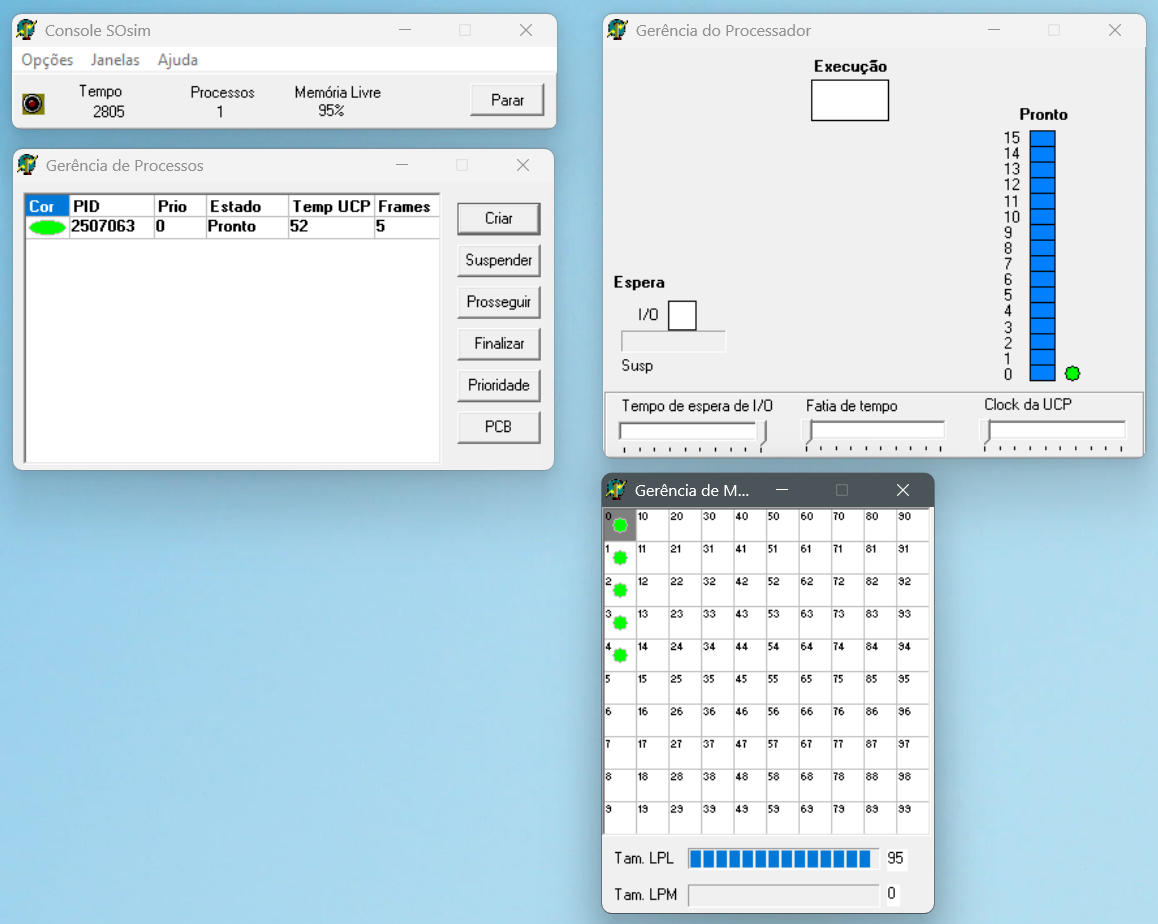
\includegraphics[scale=0.4]{../fig/fig1.png}
    \caption{Tela inicial da aplicação}
    \label{fig1}
\end{figure}

\subsubsection[]{Análise prática}
Verificável pela figura \ref{fig2} e \ref{fig3}.
\begin{figure}[htbp]
    \centering
    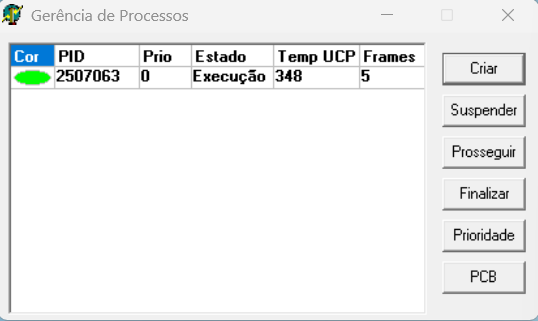
\includegraphics[scale=0.8]{../fig/fig2.png}
    \caption{Janela de processos}
    \label{fig2}
\end{figure}

\begin{figure}[htbp]
    \centering
    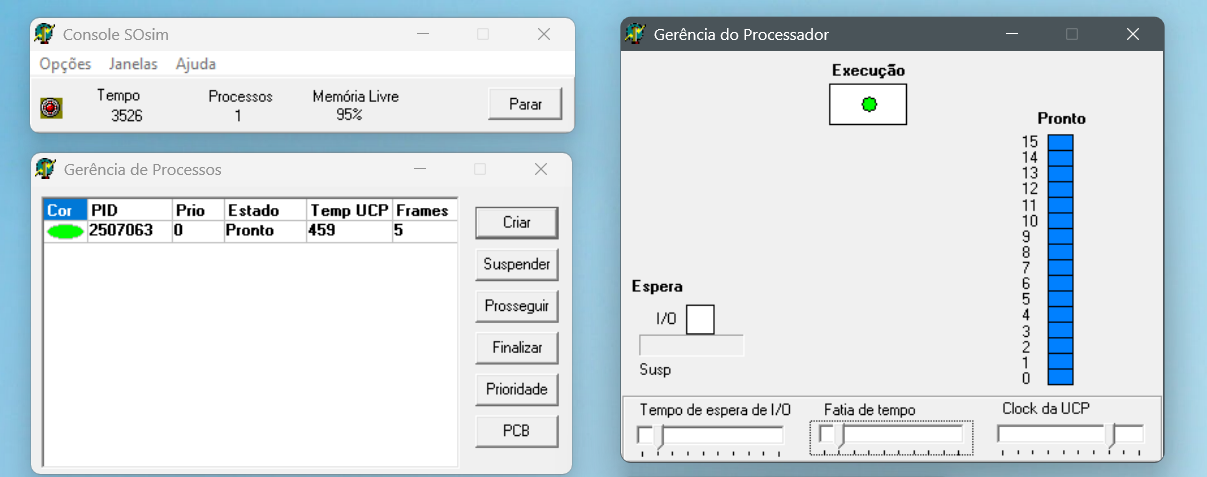
\includegraphics[scale=0.4]{../fig/fig3.png}
    \caption{Janelas do SOSim}
    \label{fig3}
\end{figure}

\subsubsection[]{Questão teórica}
No caso do gerenciador de processos, conforme sua característica, é CPU-Bound devido ao fato de que os processos ficam
em execução por muitos ciclos de clock.
\subsection[]{Tipos de processos}
\subsubsection[]{Práticas de simulação}
Verificável pela figura \ref{fig4}.
\begin{figure}[htbp]
    \centering
    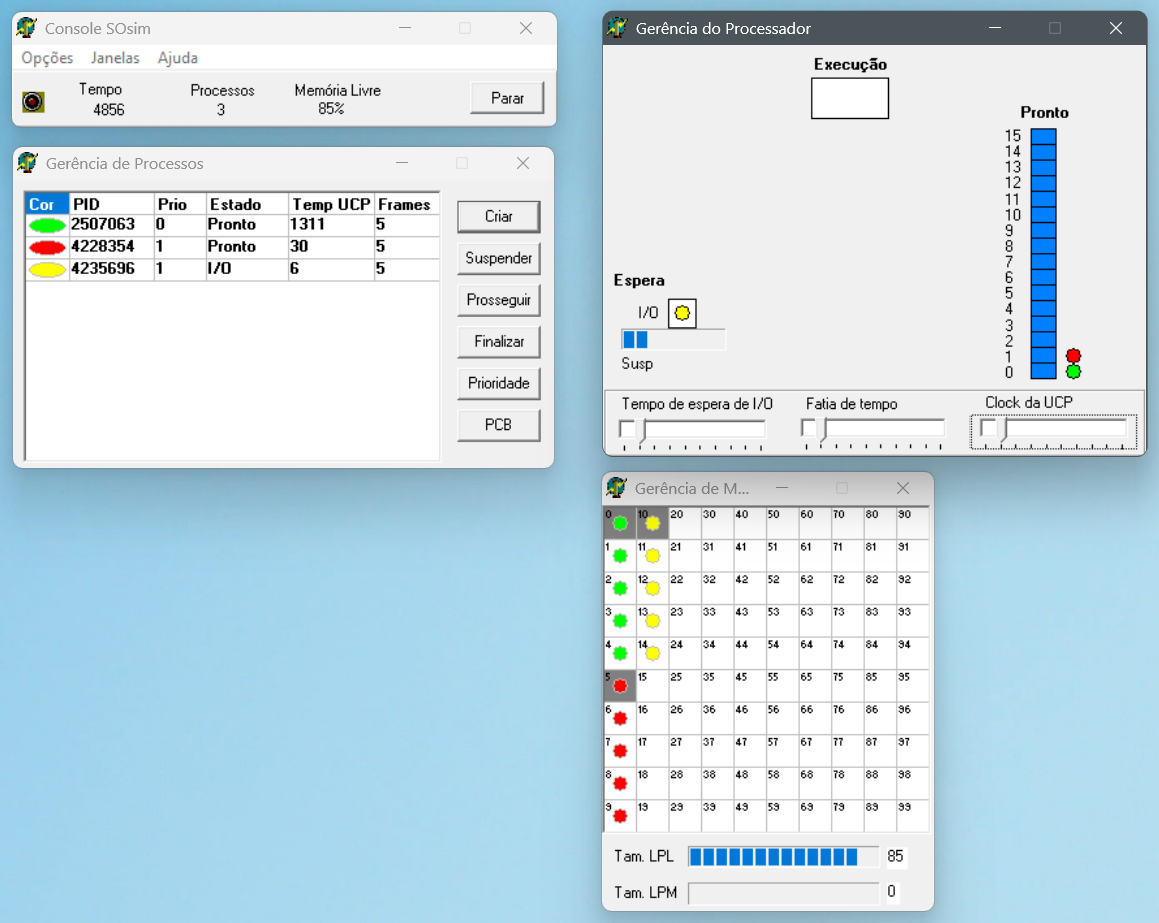
\includegraphics[scale=0.4]{../fig/fig4.png}
    \caption{Janela de processador}
    \label{fig4}
\end{figure}

\subsubsection[]{Análise prática}
Pode ser analisada conforme \ref{fig4}.
\subsubsection[]{Questão teórica}
Conforme podemos verificar no escalonamento de processos, os processos I/O-Bound tendem a ficar mais tempo em execução,
de forma que os processos de mesma prioridade, sendo do tipo CPU-Bound ficam mais tempo em espera.
\subsection[]{PCB}
\subsubsection[]{Práticas de simulação}
Verificável pela figura \ref{fig5}.
\begin{figure}[htbp]
    \centering
    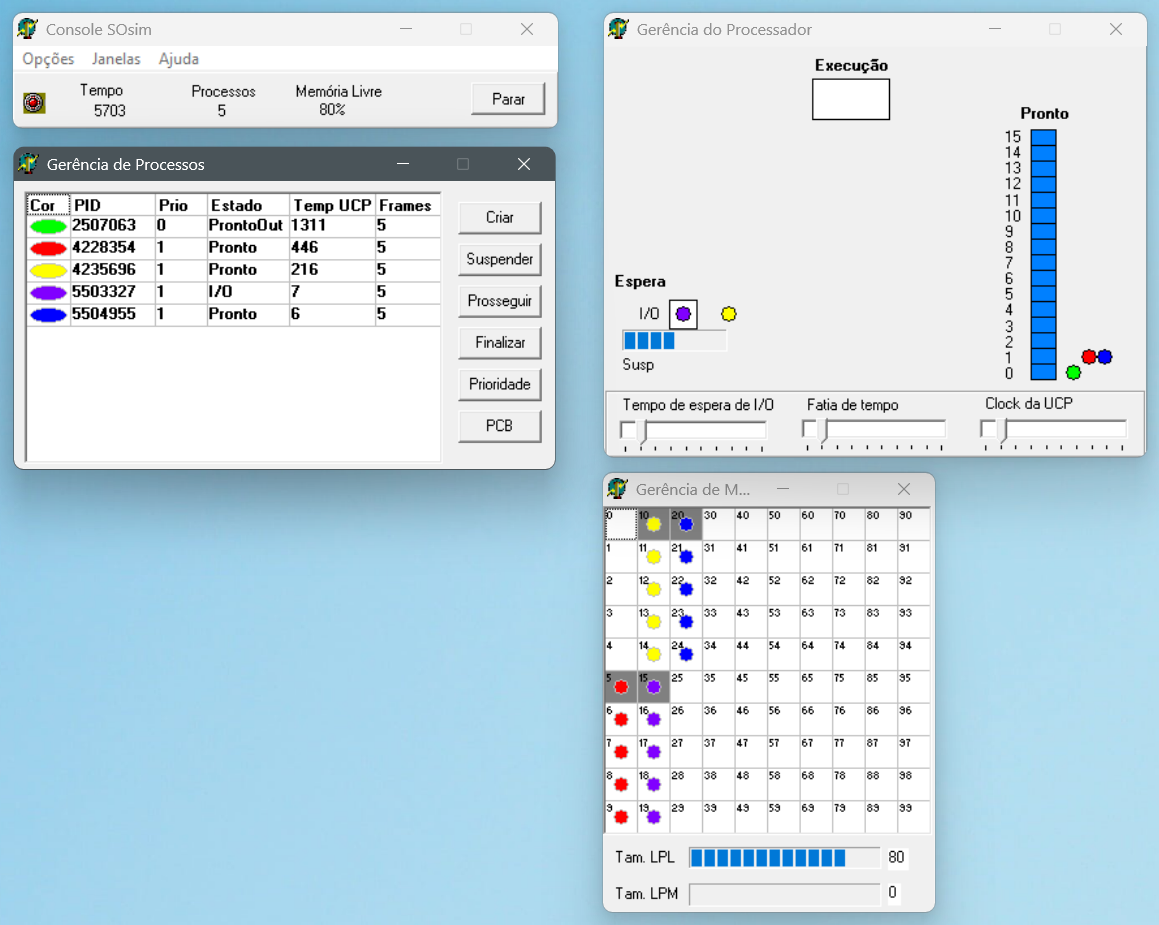
\includegraphics[scale=0.4]{../fig/fig5.png}
    \caption{Janelas do SOSim}
    \label{fig5}
\end{figure}
\subsubsection[]{Análise prática}
Verificável pela figura \ref{fig5}.
\subsubsection[]{Questão teórica}
No contexto de escalonamento de processos, muito possivelmente este ocorrido, se deve ao fato de ao criar dois processos
de igual maneira, possívelmente estes também têm mesma prioridade e tipo, logo, quando os de mesma prioridade são concluídos,
existe um espaço de tempo, em que o SO vai em busca de processos em outra prioridade, mas como não encontra, volta para à
executar os processos anteriores.
\subsection[]{Estatísticas}
\subsubsection[]{Práticas de simulação}
Verificável pela figura \ref{fig6}.
\begin{figure}[htbp]
    \centering
    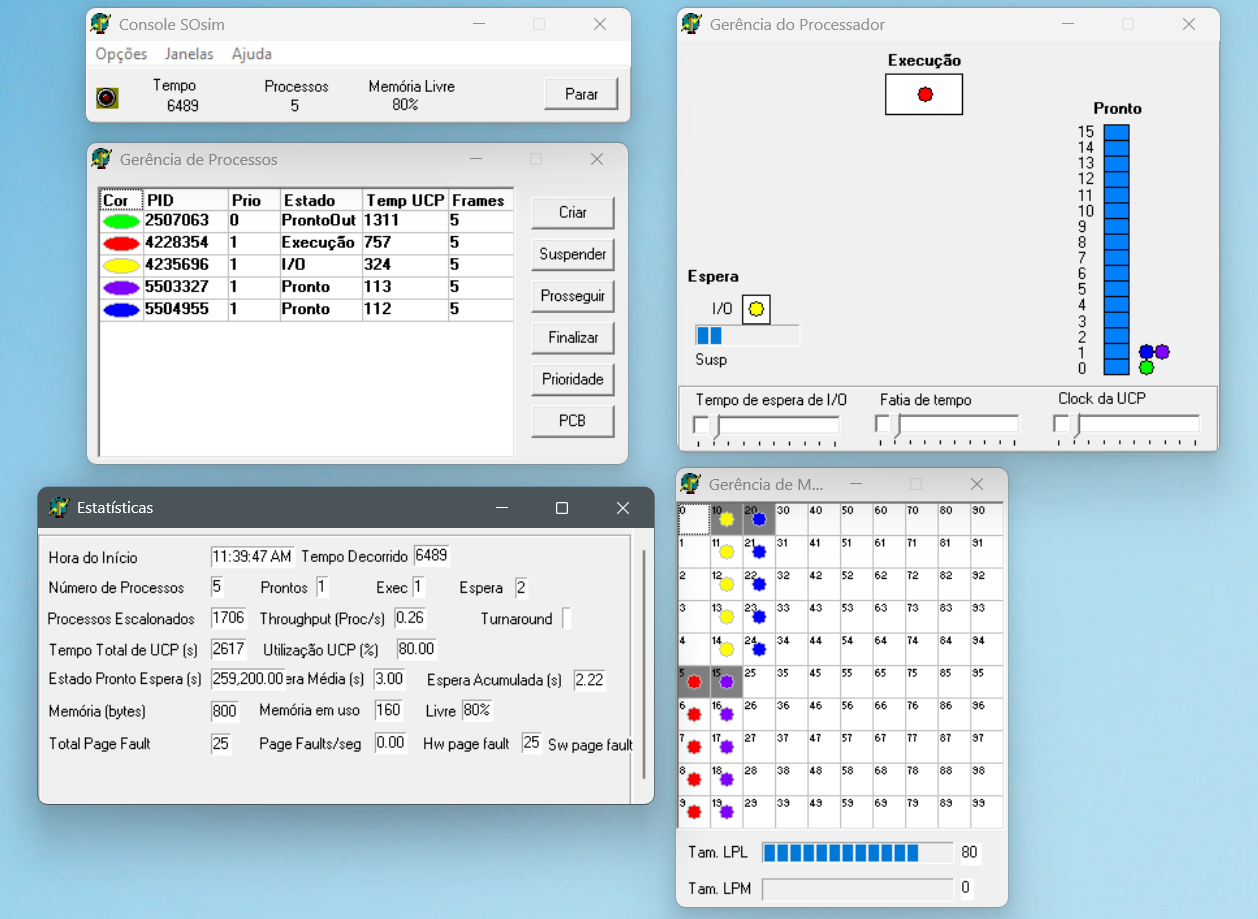
\includegraphics[scale=0.4]{../fig/fig6.png}
    \caption{Janelas do SOSim}
    \label{fig6}
\end{figure}
\subsubsection[]{Análise prática}
Verificável pela figura \ref{fig6}.
\subsubsection[]{Questão teórica}
Neste caso, ainda conforme o caso anterior, podemos verificar que isso se deve ao fato de que os processos de mesma prioridade
ainda mantêm a característica do escalonamento que leva à serem executados e posteriormente, após um tempo em espera conforme
o ciclo de estados da thread a serem executados novamente.
\subsection[]{Log de execução de processos}
\subsubsection[]{Práticas de simulação}
Verificável pela figura \ref{fig7}.
\begin{figure}[htbp]
    \centering
    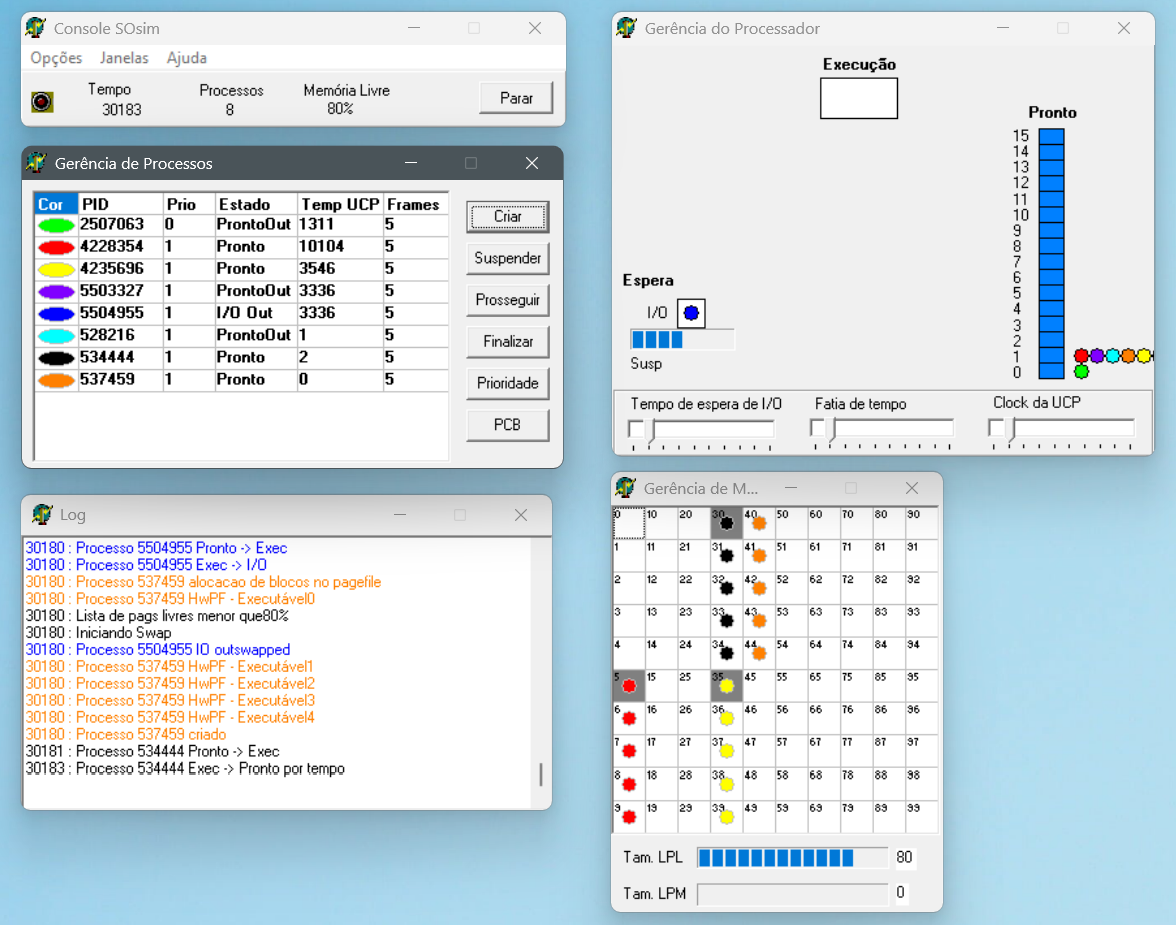
\includegraphics[scale=0.4]{../fig/fig7.png}
    \caption{Janelas do SOSim}
    \label{fig7}
\end{figure}
\subsubsection[]{Análise prática}
Verificável pela figura \ref{fig8}.
\begin{figure}[htbp]
    \centering
    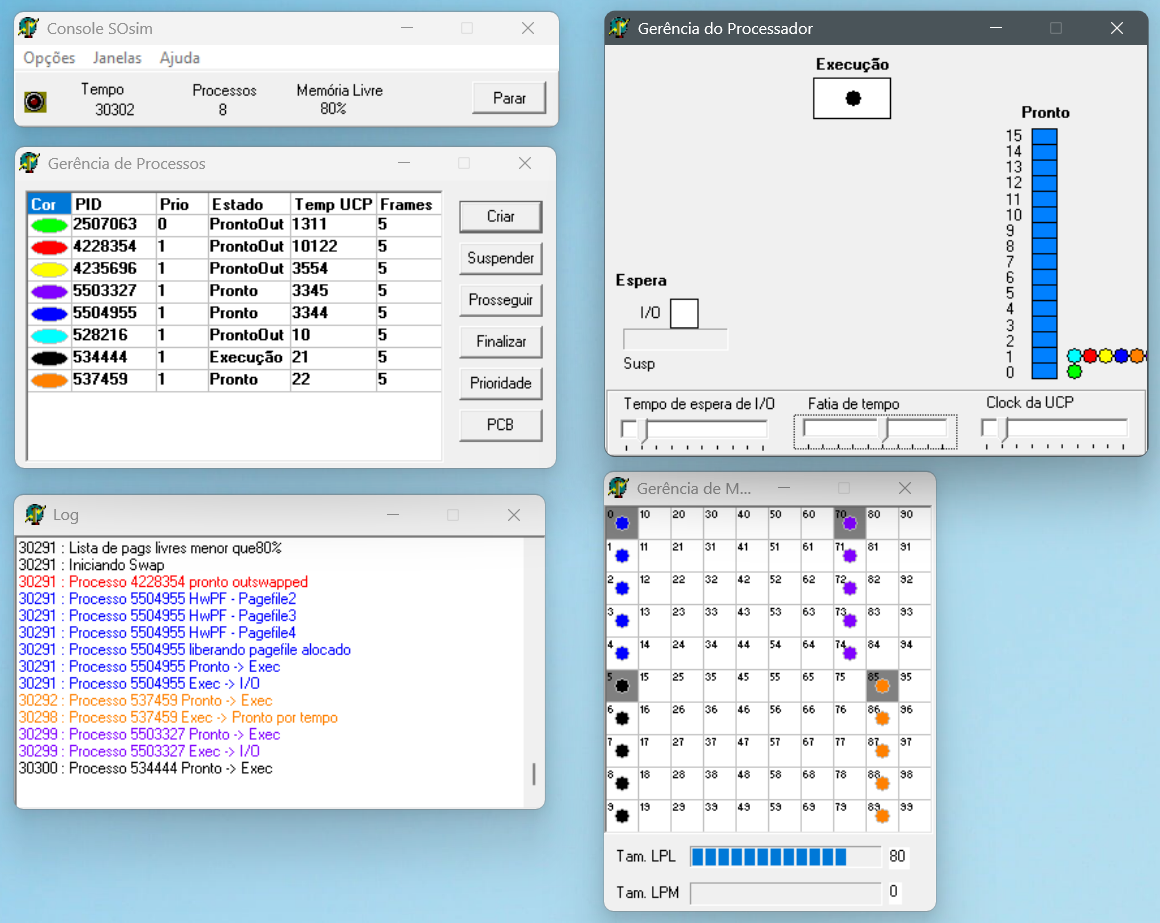
\includegraphics[scale=0.4]{../fig/fig8.png}
    \caption{Janelas do SOSim}
    \label{fig8}
\end{figure}
\subsubsection[]{Questão teórica}
Ocorre de forma que os valores de tempo fazem com que haja diferenciação no escalonamento de processos, de forma à variar
o método de escalonamento, e conforme o Log de processos, o tempo de execução em CPU dos processos.
\subsection[]{Suspensão e eliminação de processos}
\subsubsection[]{Questão teórica}
Verificável pela figura \ref{fig9}.
\begin{figure}[htbp]
    \centering
    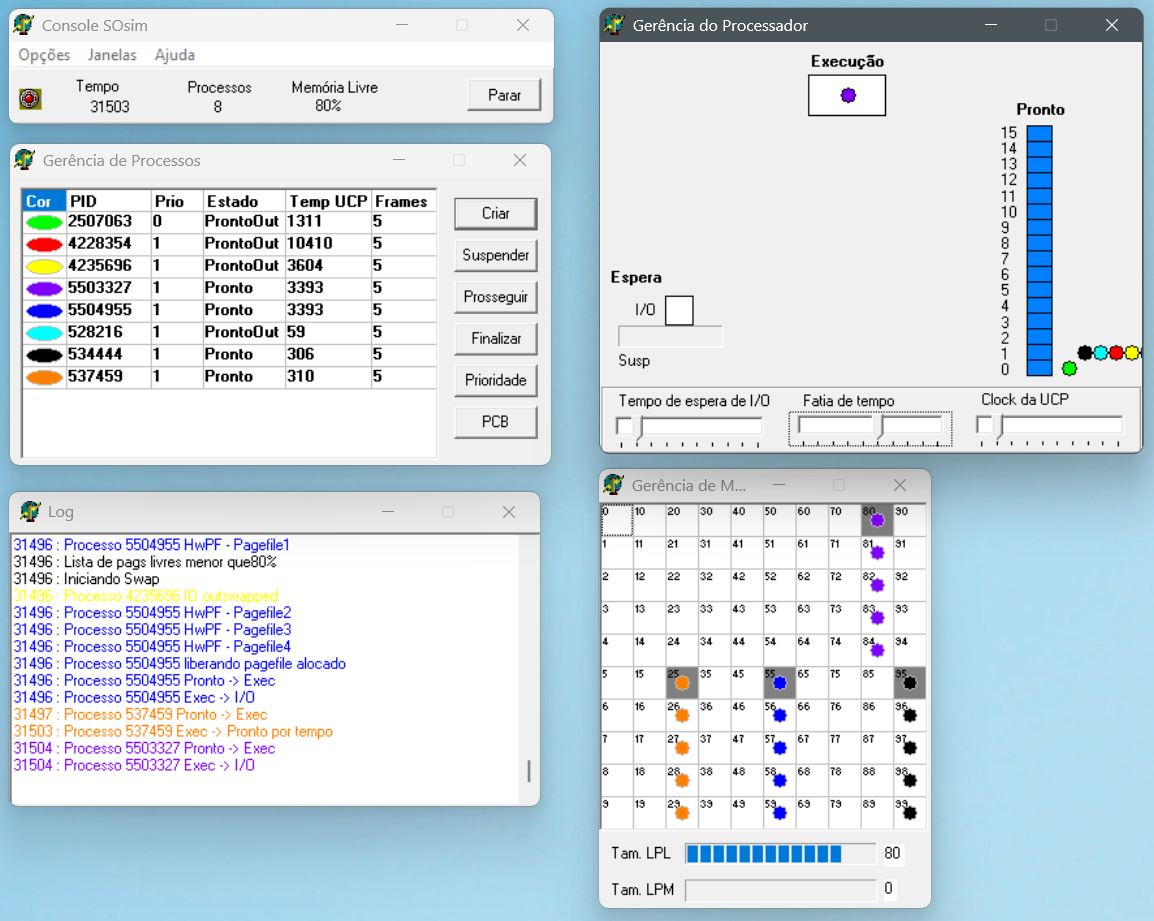
\includegraphics[scale=0.4]{../fig/fig9.png}
    \caption{Janelas do SOSim}
    \label{fig9}
\end{figure}

Verificável pela figura \ref{fig10}.
\begin{figure}[htbp]
    \centering
    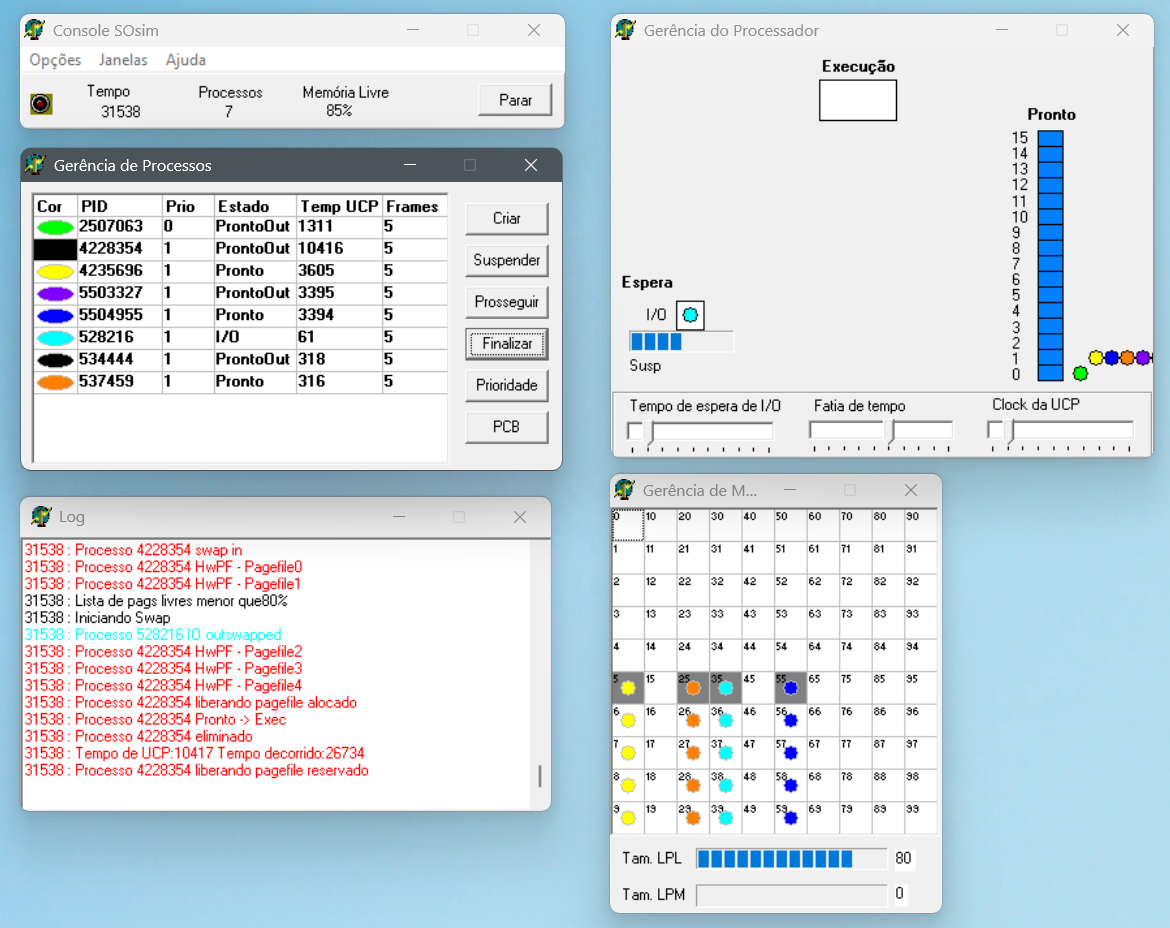
\includegraphics[scale=0.4]{../fig/fig10.png}
    \caption{Janelas do SOSim}
    \label{fig10}
\end{figure}

Ocorre que dentro do ciclo de possíveis estados de uma thread, após finalizada, sai da pilha de execução de processos,
e por fim, a excluímos.
%%%%%%%%%%%%%%%%%%%%%%%%%%%%%%%%%%%%%%%%%%%%%%%%
% Referências e Bibliografia
%%%%%%%%%%%%%%%%%%%%%%%%%%%%%%%%%%%%%%%%%%%%%%%%

\clearpage
\printbibliography

\end{document}
